%\documentclass[referee]{aa} % for a referee version
%\documentclass[onecolumn]{aa} % for a paper on 1 column  
%\documentclass[longauth]{aa} % for the long lists of affiliations 
%\documentclass[letter]{aa} % for the letters 
\documentclass{aa}

\usepackage{txfonts}
\usepackage{natbib}

\usepackage{graphicx}

\usepackage{color}
\usepackage{hyperref}
\hypersetup{colorlinks=true,allcolors=[rgb]{0,0,0.8}}

\usepackage{xcolor,soul}
\sethlcolor{yellow}
\usepackage{showyourwork}

% the three lines suppress the hyperref 'link empty' warnings
% explanation at: https://tex.stackexchange.com/questions/345764/journal-class-shows-package-hyperref-warning-suppressing-link-with-empty-targe
\makeatletter
\renewcommand*\aa@pageof{, page \thepage{} of \pageref*{LastPage}}
\makeatother

% text highlighting
\usepackage{soul}
\sethlcolor{yellow}



\begin{document} 
\authorrunning{Kenworthy et al.}
\titlerunning{ERIS gvAPP}
  \title{The ERIS gvAPP Coronagraph: theoretical and on-sky performance}

   \author{M. A. Kenworthy
          \inst{1}
          \and
          F. Dannert
          \inst{2}
          \and
          J. Hayoz
          TBD
          \inst{2}
          \and
          D. Doelman
          \inst{1}
          \and
          F. Snik
          \inst{1}
        \and
        S. Quanz
        \inst{2}
          }

   \institute{Leiden Observatory, University of Leiden,
   PO Box 9513, 2300 RA Leiden, The Netherlands\\
   \email{kenworthy@strw.leidenuniv.nl} \\
   \and 
      ETH Zurich, Switzerland
}
   \date{Received \today; accepted XXXX}

% \abstract{}{}{}{}{} 
% 5 {} token are mandatory
 
  \abstract
  % context heading (optional)
  % {} leave it empty if necessary  
   {}
  % aims heading (mandatory)
   {We describe the gvAPP coroangraph for ERIS.}
  % methods heading (mandatory)
   {On sky observations from the commissioning run enabled characterisation of the gvAPP performance.}
  % results heading (mandatory)
   {Excellent matching with the prescribed pattern.
   %
   Different wavelength performance.}
  % conclusions heading (optional), leave it empty if necessary 
   {}

   \keywords{instrumentation -- coronagraphs}

   \maketitle
%
%-------------------------------------------------------------------

   \section{Introduction}

%\begin{figure}
%%    \begin{centering}
 %   \includegraphics[width=0.5\textwidth]{figures/gvapp_psf.pdf}
 %   \caption{gvAPP psf as seen in ERIS.
%              }
%    \label{fig:erisapp}
%    \script{plot_eris_gvapp_psf.py}
%    \end{centering}
%\end{figure}
The Enhanced Resolution Imager and Spectrograph for the VLT \citep[ERIS; ][]{2023A&A...674A.207D} is an diffraction limited 1.5 to 5 micron imager and spectrograph, providing a 20 arcsecond field of view and $R=5000$ spectroscopy using an integral field unit.
%
It is composed of two parts, the integral field spectrograph SPIFFIER (REF) and the diffraction-limited high angular resolution imager NIX (REF).



\section{Phase pattern design}

\hl{MAK, DD}

Phase pattern

The goal IWA, OWA, contrast level

determining the separation of the PSFs

\section{Optical construction of the gvAPP}

\hl{MAK, DD}

Optical layering

Flatness

Wedge

Glue transmission

subsection{Compared with cryogenic tests}

\hl{MAK, DD}

Anne Boehle discussion from her paper

XXX TAKEN from ANNA's PAPER! This is David's original image...

Look at this photograph... Figure~\ref{fig:sim_results}.

Glue throughput curve

Total throughput curve

\begin{figure*}
    \centering
    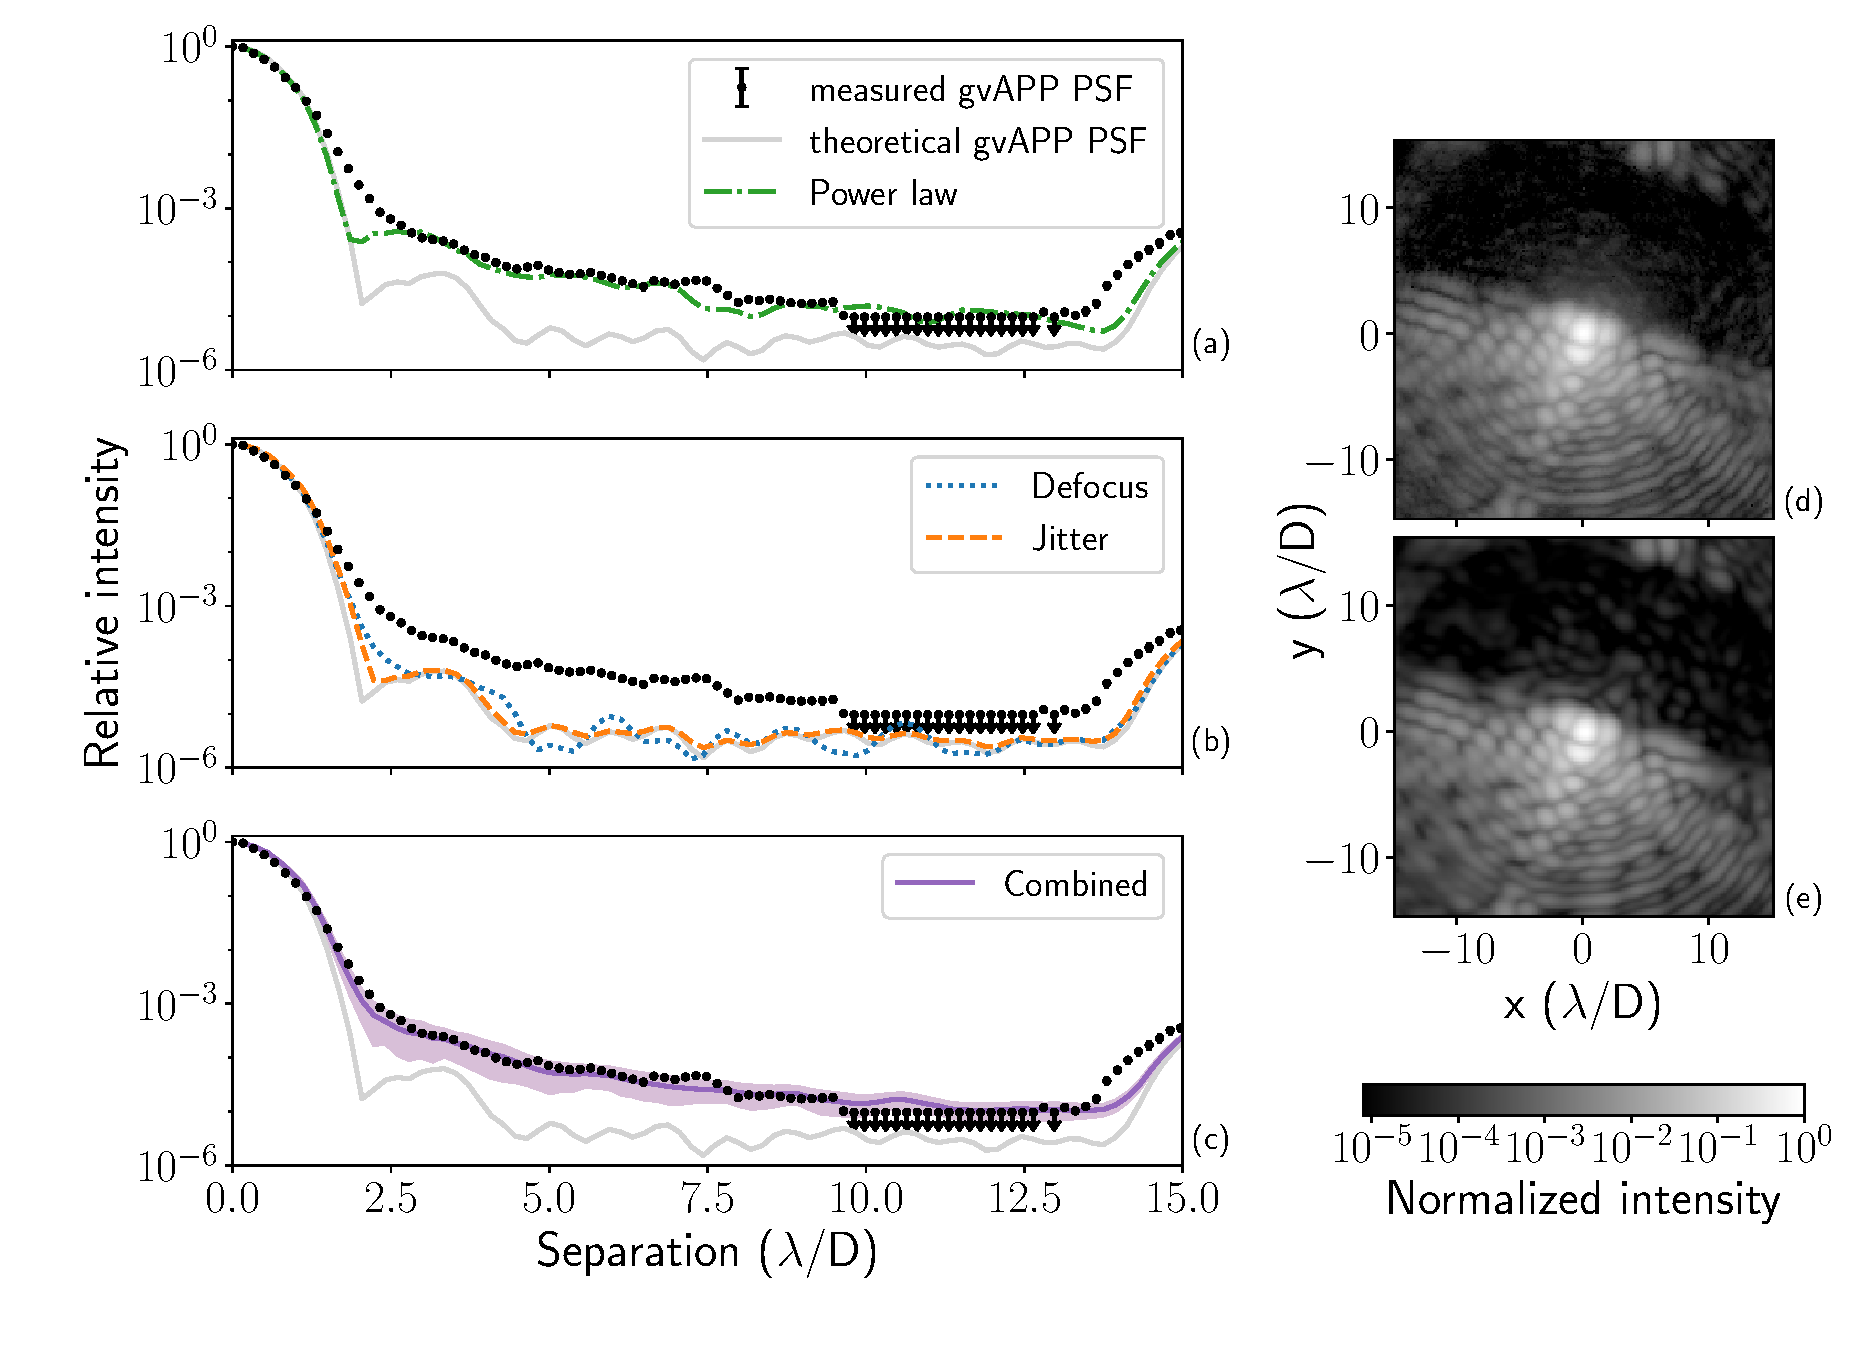
\includegraphics[width=0.95\textwidth]{figures/contrast_curve_withpsfs.pdf}
    \caption{Results from the simulations of the aberrations  observed in the gvAPP PSF.
    %
    The left column displays the simulated contrast curves when applying a a single realization of a power law aberration to simulate polishing errors (panel a), defocus and jitter aberrations (panel b), and all 3 aberrations combined including the average of 100 power law realizations and the 1$\sigma$ spread (panel c).
    %
    Each simulated contrast curve is compared to the data (black points) and to the theoretical gvAPP PSF (gray line).
    %
    The right column shows the test bench data of the left gvAPP PSF (panel d) compared to the simulated PSF with all 3 aberrations included (panel e).
    %
    We find that including polishing errors adds flux to the gvAPP dark hole as seen in the test bench measurements and that adding defocus and jitter smooths the PSF and makes the inner and outer edges of the dark hole line up with the measurements.
    %
    The combination of all three aberrations can explain the data very well in terms of the contrast curve and the PSF morphology.}
    \label{fig:sim_results}
\end{figure*}




\section{On-sky PSF comparison with model PSF}

\


\subsection{narrow band PSF on-sky}

\hl{JH, FD}

\subsection{IB on sky}

JH, FD

TODO MAK to ping Ben for K band ERIS gvAPP to get the contrast there.

left/right PSF brightness is not the same. hints at circular instrumentation systematics in ERIS???

Structure in the telescope pupil shows striping simialt to the grating for the gvAPP - some weird polarization structure in there.

\subsection{Wavelength performance predicted and measured}
\hl{JH, FD, MAK}

\section{Contrast curves}

\subsection{Current measured on-sky}
\hl{JH, FD, DD}

\subsection{Predicted performance for broad bands}
\hl{JH, FD, DD}

%------------------------
\section{Conclusions}\label{sec:conclusion}

\subsection{Impact on future designs for ELT class telescopes}

Ask Olivier and Gilles

\hl{Everyone!}

Minimise the number of glue layers (2 is probably minimum)



\begin{acknowledgements}

ADD YOUR ACKNOWLEDGEMENTS HERE

This research has used the SIMBAD database, operated at CDS, Strasbourg, France \citep{wenger2000}.
%
This work has used data from the European Space Agency (ESA) mission {\it Gaia} (\url{https://www.cosmos.esa.int/gaia}), processed by the {\it Gaia} Data Processing and Analysis Consortium (DPAC, \url{https://www.cosmos.esa.int/web/gaia/dpac/consortium}).
%
Funding for the DPAC has been provided by national institutions, in particular the institutions participating in the {\it Gaia} Multilateral Agreement.
%
To achieve the scientific results presented in this article we made use of the \emph{Python} programming language\footnote{Python Software Foundation, \url{https://www.python.org/}}, especially the \emph{SciPy} \citep{virtanen2020}, \emph{NumPy} \citep{numpy}, \emph{Matplotlib} \citep{Matplotlib}, \emph{emcee} \citep{foreman-mackey2013}, and \emph{astropy} \citep{astropy_1,astropy_2} packages.
%
\end{acknowledgements}

\bibliographystyle{aa}
\bibliography{bib}

\end{document}
